\documentclass[letterpaper]{article}
\usepackage{tikz}
% Set tiny margins so it fits on one sheet
\usepackage[top=10mm,left=5mm]{geometry}
\usetikzlibrary{calendar}
\begin{document}
% No page numbers
\pagestyle{empty}
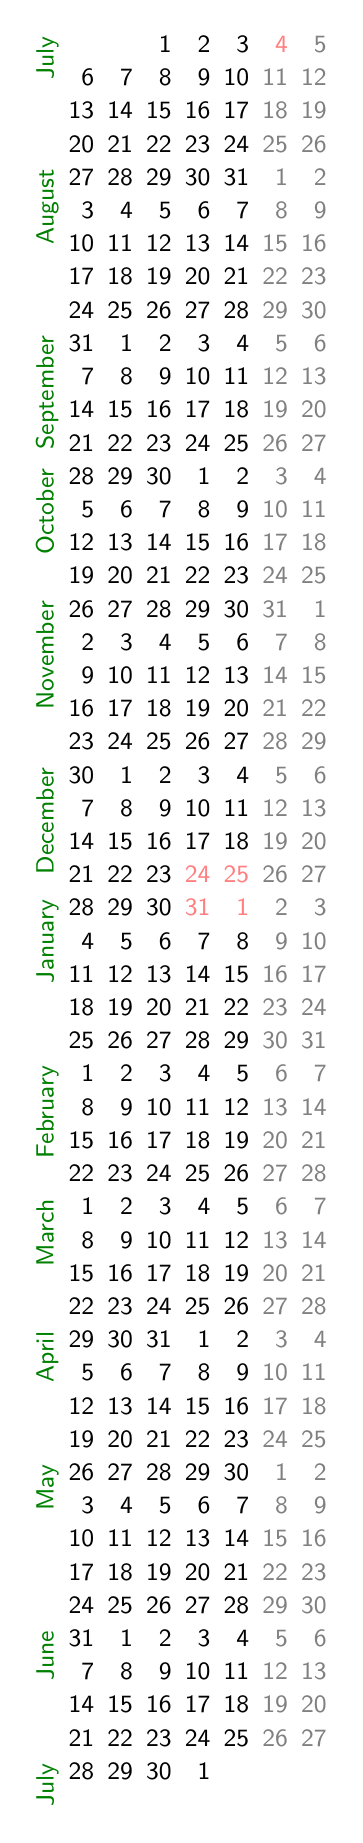
\begin{tikzpicture}
\small\sffamily
\colorlet{darkgreen}{green!50!black}
% Create a running 12 month calendar starting from the current month
\calendar[dates=\year-\month-01 to \year-\month-01+365,week list,
month label left vertical,month yshift=0pt,
month text=\textcolor{darkgreen}{\%mt}]
if (weekend) [black!50]
% Regular holidays are red
if (equals=01-01,
    equals=07-04,
    equals=12-24,
    equals=12-25,
    equals=12-31]) [red!50]
% Holidays that vary by year are red
if (equals=2012-04-06,
    equals=2012-04-08,
    equals=2012-05-28,
    equals=2012-09-03,
    equals=2012-11-22, 
    equals=2012-12-26,
    equals=2012-12-27,
    equals=2012-12-28) [red!50]
if (equals=2013-01-21,
    equals=2013-03-29,
    equals=2013-03-31,
    equals=2013-05-27,
    equals=2013-09-02,
    equals=2013-11-28,
    equals=2013-11-29, 
    equals=2013-12-26,
    equals=2013-12-27,
    equals=2013-12-30) [red!50]
if (equals=2014-01-20,
    equals=2014-04-18,
    equals=2014-04-20,
    equals=2014-05-26,
    equals=2014-09-01,
    equals=2014-11-27,
    equals=2014-11-28,
    equals=2014-12-26,
    equals=2014-12-29,
    equals=2014-12-30) [red!50];
\end{tikzpicture}
\end{document}
